\chapter{Q-Factor}
\section{Reference Ideas}



\subsection{Ideas}
%The ultrasound method \cite{Foiret2014} enables the simultaneous measurement of cortical thickness and tissue elastic properties where previous techniques such as DXA (the \textit{de facto} method) could archieve.
As studied before, factors of risk fracture are the thickness, porosity and particular quality elements of the extracelular matrix as explained in \cite{Bernard2015}. The QUS method \cite{Foiret2014}, \cite{Minonzio2018} of axial transmission technique is based on recording from the propagation of guided waves over the media, were damping factors affect the signal. This is associated to a viscoelastic behavior of the cortical bone arrising mainly from the presence of collagen fibers, specifically treated with Resonant Ultrasound Spectroscopy techniques. Thus, its natural to study the correspondence between such damping elements and their preponderance on the resulting homogenized coefficients by the two-scale homogenization theory

\textit{Bernard} \textit{et al. }\cite{Bernard2015} studied in a viscoelastic behavior on a frequency domain model of bone their results, in which he modelled the elastic tensor $C^*_{ij}$ with damping effect given by:
\begin{equation*}
C^*_{ij} = C_{ij} + i C_{ij}^{'} = C_{ij} (1+ iQ_{ij}^{-1})
\end{equation*}

where the $Q^{-1}_{ij}$ are defined as ratios of the imaginary part ($C_{ij}'$) to the real part ($C_{ij}$), denoting the so-called quality factors.

In this section, I shall formulate such quality factors following the two-scale homogenization formalism, recovering the homogenized coefficients in the elastic case at different porosity levels and particularly obtaining prediction for the quality factors at some interval. Under the actual literature, such coefficients are yet to be validated since there isn't enough experimental literature to confirm our predictions.


\section{Workflow for the Q-factor}
The idea for this section is to formalize the Q-factor in the framework of homogenized equations.
In this case, we will give a definition for the Q-factor from a elastodynamic Kelvin-Voigt model of bone.\\
More specifically, we define the mechanical behavior of bone as a multiphase viscoelastic material composed of two-phases with cell unit in the form $\mathbf{Y} = Y_{m} \cup Y_{f}$ being the matrix and fluid parts respectively.
For the bone matrix, we associate an elastic behavior defined by the elastic coefficient:
\begin{equation*}
    C_{ijkl}(\mathbf{y}) = C_{ijkl}^m \mathbb{I}_{Y_m}(\mathbf{y}) + C_{ijkl}^f \mathbb{I}_{Y_f}(\mathbf{y})
\end{equation*}
while the bone marrow is defined modelled as the viscous part, associated to a coefficient given in the form:
\begin{equation*}
    D_{ijkl}(\mathbf{y}) =  D_{ijkl}^m \mathbb{I}_{Y_m}(\mathbf{y}) + D_{ijkl}^f \mathbb{I}_{Y_f}(\mathbf{y})
\end{equation*}
Moreover, the relations between both coefficients is given as an attenuation specified by parameters $\epsilon^{(m)}, \epsilon^{(f)} >0$ associated to the bone matrix and marrow respectively. Explicitely, we assume then:
\begin{equation*}
    D_{ijkl}^m(\mathbf{y}) = \epsilon^{(m)} C_{ijkl}^m(\mathbf{y}) , \quad D_{ijkl}^f (\mathbf{y}) = \epsilon^{(f)} C_{ijkl}^f(\mathbf{y})
\end{equation*}


\begin{rem}
By fixing this kind of relation, the idea is to obtain a model of viscoelasticity in which the viscous part can be modelled by a linear attenuation of the elastic one, so that the overall behavior is transverse isotropic defined with just a pair of parameters $(\epsilon^m, \epsilon^w)$ that mimic closely the experimental behavior of bone.
\end{rem}

\subsection{Workflow}
\begin{rem}
For the case of 2D modelling of transverse isotropic material, the simulated solutions are close enough to \textit{Parnel and Grimal} prediction with their approximation method.
\end{rem}
In time domain, we consider an elastodynamic model of Kelvin-Voigt type behavior with mixed boundary conditions, described in the form:
\begin{equation*}
    \left \{
    \begin{array}{cc}
        \rho^{\epsilon}\partial_{tt}u - \nabla \cdot \sigma(u, \partial_t u) = \mathbf{0} & \text{ in } (0,T)\times \Omega \\
        \sigma^{\epsilon}(u,\partial_t u)  = \mathbf{C}:\mathbf{e}(u) + \mathbf{D}:\mathbf{e}(\partial_t u) & \text{ in } (0,T)\times\Omega \\
        \sigma^{\epsilon}(u, \partial_t u)\cdot n = \mathbf{F} & \text{ on }(0,T)\times \Gamma_N \\ 
        u = \mathbf{0} & \text{ on } (0,T)\times \Gamma_D
    \end{array}
    \right .
\end{equation*}
\begin{rem}
In the above and the next developments, we assume resting initial conditions, i.e., $\partial_t u = u = \mathbf{0}$, not written explicitly in the models and deduction.
\end{rem}
Using now the fourier transform defined at frequency $\omega \in \mathbb{R}$ with base $\{e^{i\omega t}\}_{\omega}$, we obtain our redefined problem in the Fourier domain given by:
\begin{equation*}
    \left \{
    \begin{array}{cc}
        -\omega^2 \rho^{\epsilon} \hat{u}^{\epsilon} - \nabla \cdot \hat{\sigma}_{\epsilon,\omega}(\hat{u}^{\epsilon}) = \mathbf{0} & \text{ in } \Omega  \\
        \hat{\sigma}_{\epsilon,\omega} (\hat{u}^{\epsilon}) = (\mathbf{C} + i\omega \mathbf{D}):\mathbf{e}(\hat{u}^{\epsilon}) & \text{ in } \Omega \\
        \hat{\sigma}_{\epsilon,\omega} (\hat{u}^{\epsilon}) \cdot n = \hat{\mathbf{F}}(\omega) & \text{ on } \Gamma_N \\
        \hat{u}^{\epsilon} = \mathbf{0} & \text{ on } \Gamma_D
    \end{array}
    \right .
\end{equation*}
such that at $\omega = 0$ we have $\hat{u}^{\epsilon}=\mathbf{0}$ at $\Omega$.\\

Now, homogenizing by using the two-scale asymptotic method, it follows for effective (macroscopic) model defined at frequency $\omega$ by:
\begin{equation*}
    \left \{
    \begin{array}{cc}
        -\omega^2 \rho^{0} \hat{u}^0 - \nabla \cdot \hat{\sigma}^0(\hat{u}^0)  = \mathbf{0} & \text{ in } \Omega \\
        \hat{\sigma}^{0} (\hat{u}^0)  = (\mathbf{C} + i\omega \mathbf{D})^{hom}:\mathbf{e}(\hat{u}^0) & \text{ in } \Omega \\
        \hat{\sigma}^{0} (\hat{u}^0) \cdot n = \hat{\mathbf{F}}(\omega) & \text{ on } \Gamma_N \\
        \hat{u}^0 = \mathbf{0} & \text{ on } \Gamma_D
    \end{array}
    \right .
\end{equation*}

In particular, the homogenized coefficients, are defined by the cell problem solutions $N^{rs} \in \mathbf{H}^1_{\#}(\mathbf{Y}, \mathbb{C})$, described for each $r,s \in \{1,2,3\}$ in the form
\begin{equation*}
    \left \{
    \begin{array}{cc}
         \partial_{y_j} \big[ \big( C_{ijkl} + i\omega D_{ijkl} \big) \mathbf{e}_{kl}(N^{rs}) \big] &= - \partial_{y_j} \big[ C_{ijkl} + i\omega D_{ijkl} \big] \quad \forall y \in \mathbf{Y} \\
        \big \langle C_{ijkl} + p D_{ijkl} \big \rangle_{\mathbf{Y}}  = 0 & 
    \end{array}
    \right.
\end{equation*}
\begin{rem}
Since the cell problems must be valid for each $\omega \in \mathbb{R}$ and for each $\mathbf{y} \in \mathbf{Y}$ we would like to decouple the cell PDE problems so that we can define a ratio viscosity-elasticity, i.e. an expression for the Q-factor.
\end{rem}
The decoupling is then defined by considering the separation between the real and imaginary parts associated to the cell solutions, i.e., by considering the decomposition
\begin{equation*}
    N^{rs}(\mathbf{y}) = \mathbf{N}_R^{rs}(\mathbf{y}) + i\mathbf{N}_I^{rs}(\mathbf{y})
\end{equation*}
being now the vectors functions $\mathbf{N}_R^{rs}, \mathbf{N}_I^{rs}$ in $\mathbf{H}^1_{\#}(\mathbf{Y},\mathbb{R})$ solving the following PDE system associated to the real and imaginary part decomposition:
\begin{equation*}
    \left \{
    \begin{array}{cc}
        \partial_{y_j} \big[ C_{ijkl} \mathbf{e}_{kl}(\mathbf{N}^{rs}_R) -\omega D_{ijkl} \mathbf{e}_{kl}(\mathbf{N}^{rs}_I) \big] = - \partial_{y_j} \big[ C_{ijrs} \big] & \forall \mathbf{y} \in \mathbf{Y} \\
        \partial_{y_j} \big[ C_{ijkl} \mathbf{e}_{kl}(\mathbf{N}^{rs}_I) +\omega D_{ijkl} \mathbf{e}_{kl}(\mathbf{N}^{rs}_R) \big] = - \partial_{y_j} \big[ \omega D_{ijrs} \big] & \forall \mathbf{y} \in \mathbf{Y} \\
        \big \langle \mathbf{N}^{rs}_R \big \rangle_{\mathbf{Y}},\big \langle \mathbf{N}^{rs}_I \big \rangle_{\mathbf{Y}} = \mathbf{0}  &
    \end{array}
    \right.
\end{equation*}
\begin{rem}
Note in particular that for the above cell problems, we existence and uniqueness of a weak solution is guaranteed since the problem can be rewritten as a fully elliptic operator, being the solution unique by applying the normalization condition on mean equal $\mathbf{0}$.
\end{rem}
With the solution to the cell problem, we can then define the homogenized coefficients associated to the elastic and viscous part by recalling first:
\begin{equation*}
    \hat{\sigma}_{ij}^0 (\hat{u}^0,\omega) = R_{ijkl}^{hom} (\omega) \mathbf{e}_{kl}(\hat{u}^0)
\end{equation*}
being the homogenized tensor
\begin{equation*}
    R^{hom}_{ijrs}= \big \langle  C_{ijrs} + i\omega D_{ijrs} + \big( C_{ijkl} + i \omega D_{ijkl} \mathbf{e}_{kl}(\mathbf{N}^{rs}) \big) \big \rangle  
\end{equation*}
so that, using the decomposition of $N^{rs}$ it follows that:
\begin{align*}
    R^{hom}_{ijrs} &= \big \langle C_{ijrs} + \big( C_{ijkl}\mathbf{e}_{kl}( \mathbf{N}^{rs}_R) -\omega D_{ijkl}\mathbf{e}_{kl}(\mathbf{N}^{rs}_I) \big) \big \rangle \\
    & \, + i \big \langle \omega D_{ijrs} + \big( C_{ijkl} \mathbf{e}_{kl}(\mathbf{N}^{rs}_I) + \omega D_{ijkl}\mathbf{e}_{kl}(\mathbf{N}^{rs}_R) \big) \big \rangle \\
    & := C^{hom}_{ijrs} + \mathbf{i} \omega D^{hom}_{ijrs}
\end{align*}

It follows in particular, the definition of the $Q_{ij}$ factor, defined directly on the tensor coefficients is given by:
\begin{equation}
    \label{Qfactor-Def}
    Q_{ijrs}^{-1}(\omega) := \frac{D^{hom}_{ijrs}(\omega)}{ C^{hom}_{ijrs}(\omega)}
\end{equation}
where the homogenized coefficients are defined as above.
Let us note the preponderant dependency of the frequency associated on the defined factor, which as study above, derives explicitly from the Kelvin-Voigt viscoelastic assumption of the mechanical model. 

An aspect that must be taken into account is the nonlinear effect produced added from the asymtotic asumption on the solution, expressed in the term $N^{rs}$ at the homogenized coefficients definition that can be explicitly stated from (\ref{Qfactor-Def}).
Its possible to account for that effect by taking a decomposition on the linear part associated to the mean over the coefficient itself and the nonlinear effect produced from the solutions to the cell problems, i.e., from (\ref{Qfactor-Def}) the decomposition in its linear and nonlinear effects its obtained as:
\begin{equation}
    \label{Expansion-Qfactor}
    \begin{aligned}
        Q_{ijrs}^{-1}  & = \frac{D_{hom}^{(0)} + D_{hom}^{(1)}}{C_{hom}^{(0)} + C_{hom}^{(1)}}  \\
         & =  \frac{D_{hom}^{(0)}}{C_{hom}^{(0)}} + \frac{1}{C^{(0)}_{hom}( C^{(0)}_{hom} + C^{(1)}_{hom}} \big[C^{(0)}_{hom} \big( D^{(0)}_{hom} + D^{(1)}_{hom}\big) - D^{(0)}\big( C^{(0)}_{hom} + C^{(1)}_{hom} \big) \big]
    \end{aligned}
\end{equation}
where its being used the notation for the linear terms in $p \in [0,1]$ (porosity) by:
\begin{equation*}
    C^{(0)}_{hom} = \langle C_{ijrs} \rangle_{\mathbf{Y}} \quad  D^{(0)}_{hom} = \langle D_{ijrs} \rangle_{\mathbf{Y}}
\end{equation*}
and the nonlinear terms with respect to $p \in [0,1]$ associated to the solutions $N^{rs}$ given by:
\begin{equation*}
    \begin{array}{cc}
        C^{(1)}_{hom} =& \langle C_{ijkl}\mathbf{e}_{kl}(N^{rs}_R) - \omega D_{ijkl}\mathbf{e}_{kl}(N^{rs}_I) \rangle_{\mathbf{Y}} \\
        D^{(1)}_{hom} =& \langle \omega^{-1} C_{ijkl}\mathbf{e}_{kl}(N^{rs}_I) + D_{ijkl}\mathbf{e}_{kl}(N^{rs}_R) \rangle_{\mathbf{Y}} 
    \end{array}
\end{equation*}

\begin{figure}[!h]
	\centering
	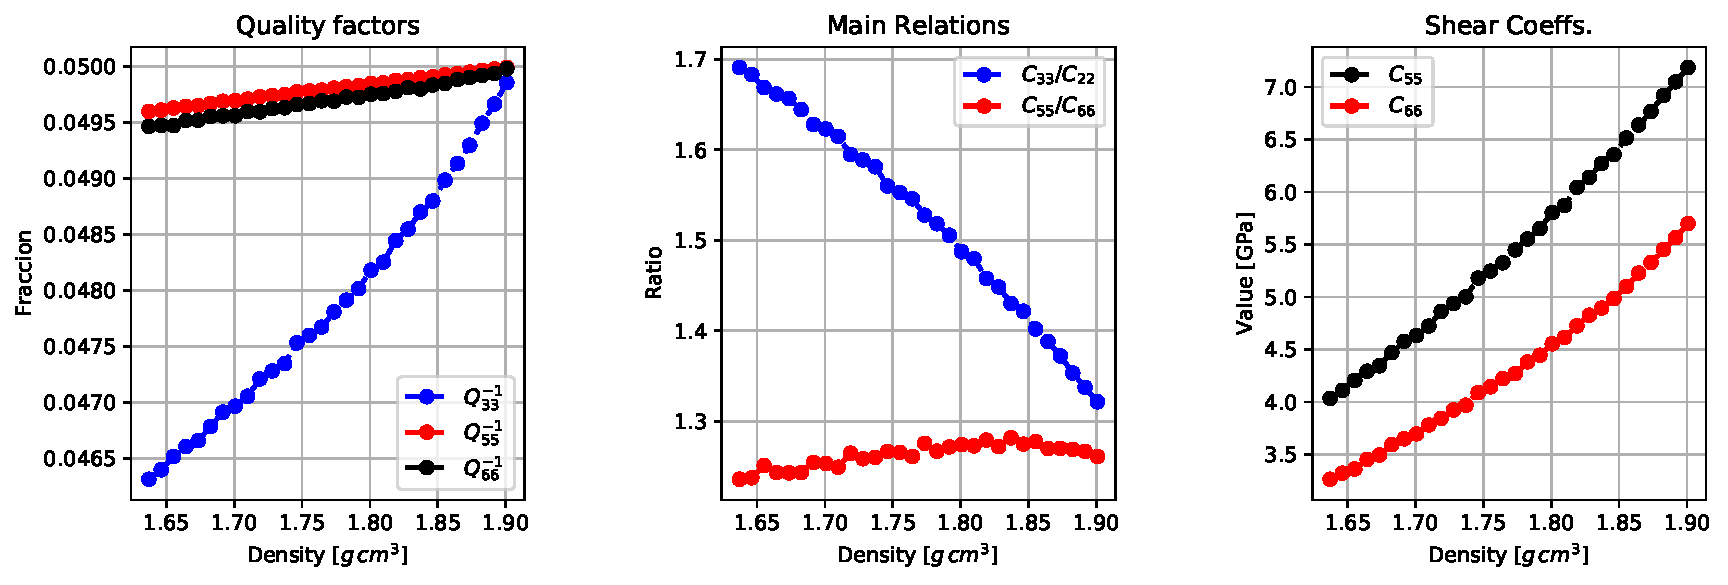
\includegraphics[width=\textwidth]{images/Qfactors/CellProb_QfactorCircular5E-2_Relations.pdf}
	\caption{Predicted Behavior for the Viscoelastic Model: Its shown on the left figure the predicted quality factors for a \textit{Kelvin-Voigt} model; the center figure a prediction of homogenized coefficient ratios, and on the right figure some homogenized shear ratios behaves as in \cite{Bernard2015} }
	\label{PredictionHomCoeffs-Qfactor}
\end{figure} 

